\section{Stack}
The stack of Mitosis consists of two main blocks. Mitosis-Core and Mitosis-Stream. Mitsois-Core is responsible to set up the overlay network and connect the peers with each other. Mitosis-Stream works on top of Mitosis-Core and provides the video streaming functionality.
Symbiosis is a sample application that uses Mitosis to realise a basic video broadcasting application.

The stack of the implementation is presented in \vref{fig:mit-stack}.

\begin{figure}
\centering
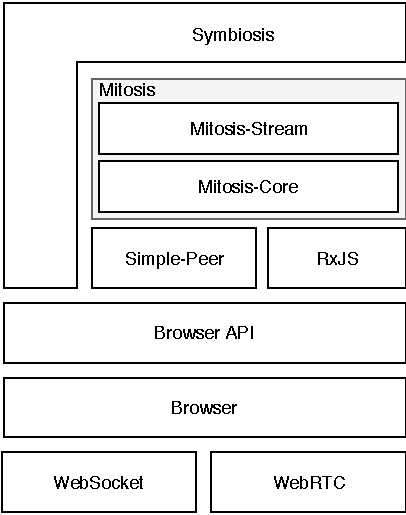
\includegraphics[width=0.7\textwidth]{graphics/implementation/mitosis-overall.pdf}
\caption{Implementation Stack}
\label{fig:mit-stack}
\end{figure}

\paragraph{Stack}
Mitosis is an SDK developed with JavaScript. Therefore, a basic requirement is a JavaScript runtime that can be either provided by a browser or by \textit{Node.js}\footnote{Node.js. URL: {https://nodejs.org}}. The primary focus of this thesis is the execution in a browser environment but Node.js support is possible.

As code dependencies it has the JavaScript library \textit{simple-peer}\footnote{simple-peer. URL: {https://github.com/feross/simple-peer}} and \textit{RxJS}\footnote{RxJS. URL: {https://rxjs.dev}}. 

simple-peer is an open source library that wraps the complex WebRTC API and provides a simpler interface, thus the name simple-peer. More importantly simple-peer provides cross-browser support and also bridges the gap between Browsers, \textit{Electron}\footnote{Electron. URL: {https://electronjs.org}} and Node.js.
The main maintainer of the library is Feross Aboukhadijeh and the library is used by a lot of other WebRTC based projects like \textit{WebTorrent}\footnote{WebTorrent. URL: {https://webtorrent.io}}.

RxJS is also open source and provides support for reactive programming. One well known supporter of RxJS is \textit{Angular}\footnote{Angular. URL: {https://angular.io}}, which is a popular JavaScript framework and provided by Google.
Mitosis uses RxJS to allow components to subscribe on other components.



